These reconstruction steps all take place before we interact with the data. The cut values in \Cref{tab:pid-cuts} are loose, and there is surely background remaining. To remove it, we first must know the potential sources of backgrounds in the $K_S^0K_S^0$ channel, which we will do by simulating a large set of events with many different reaction topologies, passing them through reconstruction, and then comparing the distributions of each topology which makes it through. The simulation uses the \texttt{bggen} Monte Carlo generator, which in turn uses \texttt{PYTHIA}~\cite{Bierlich2022} for event generation and a GlueX implementation of \texttt{Geant4}~\cite{Allison2006,Allison2016,Agostinelli2003}. The relative proportions of reaction topologies do not necessarily reflect the production cross sections we expect to see in data (for instance, there are no resonances included in the $K_S^0K_S^0$ channel), but they should give us a good idea of the kinds of topologies which leak into this channel.

\begin{figure}
  \begin{center}
    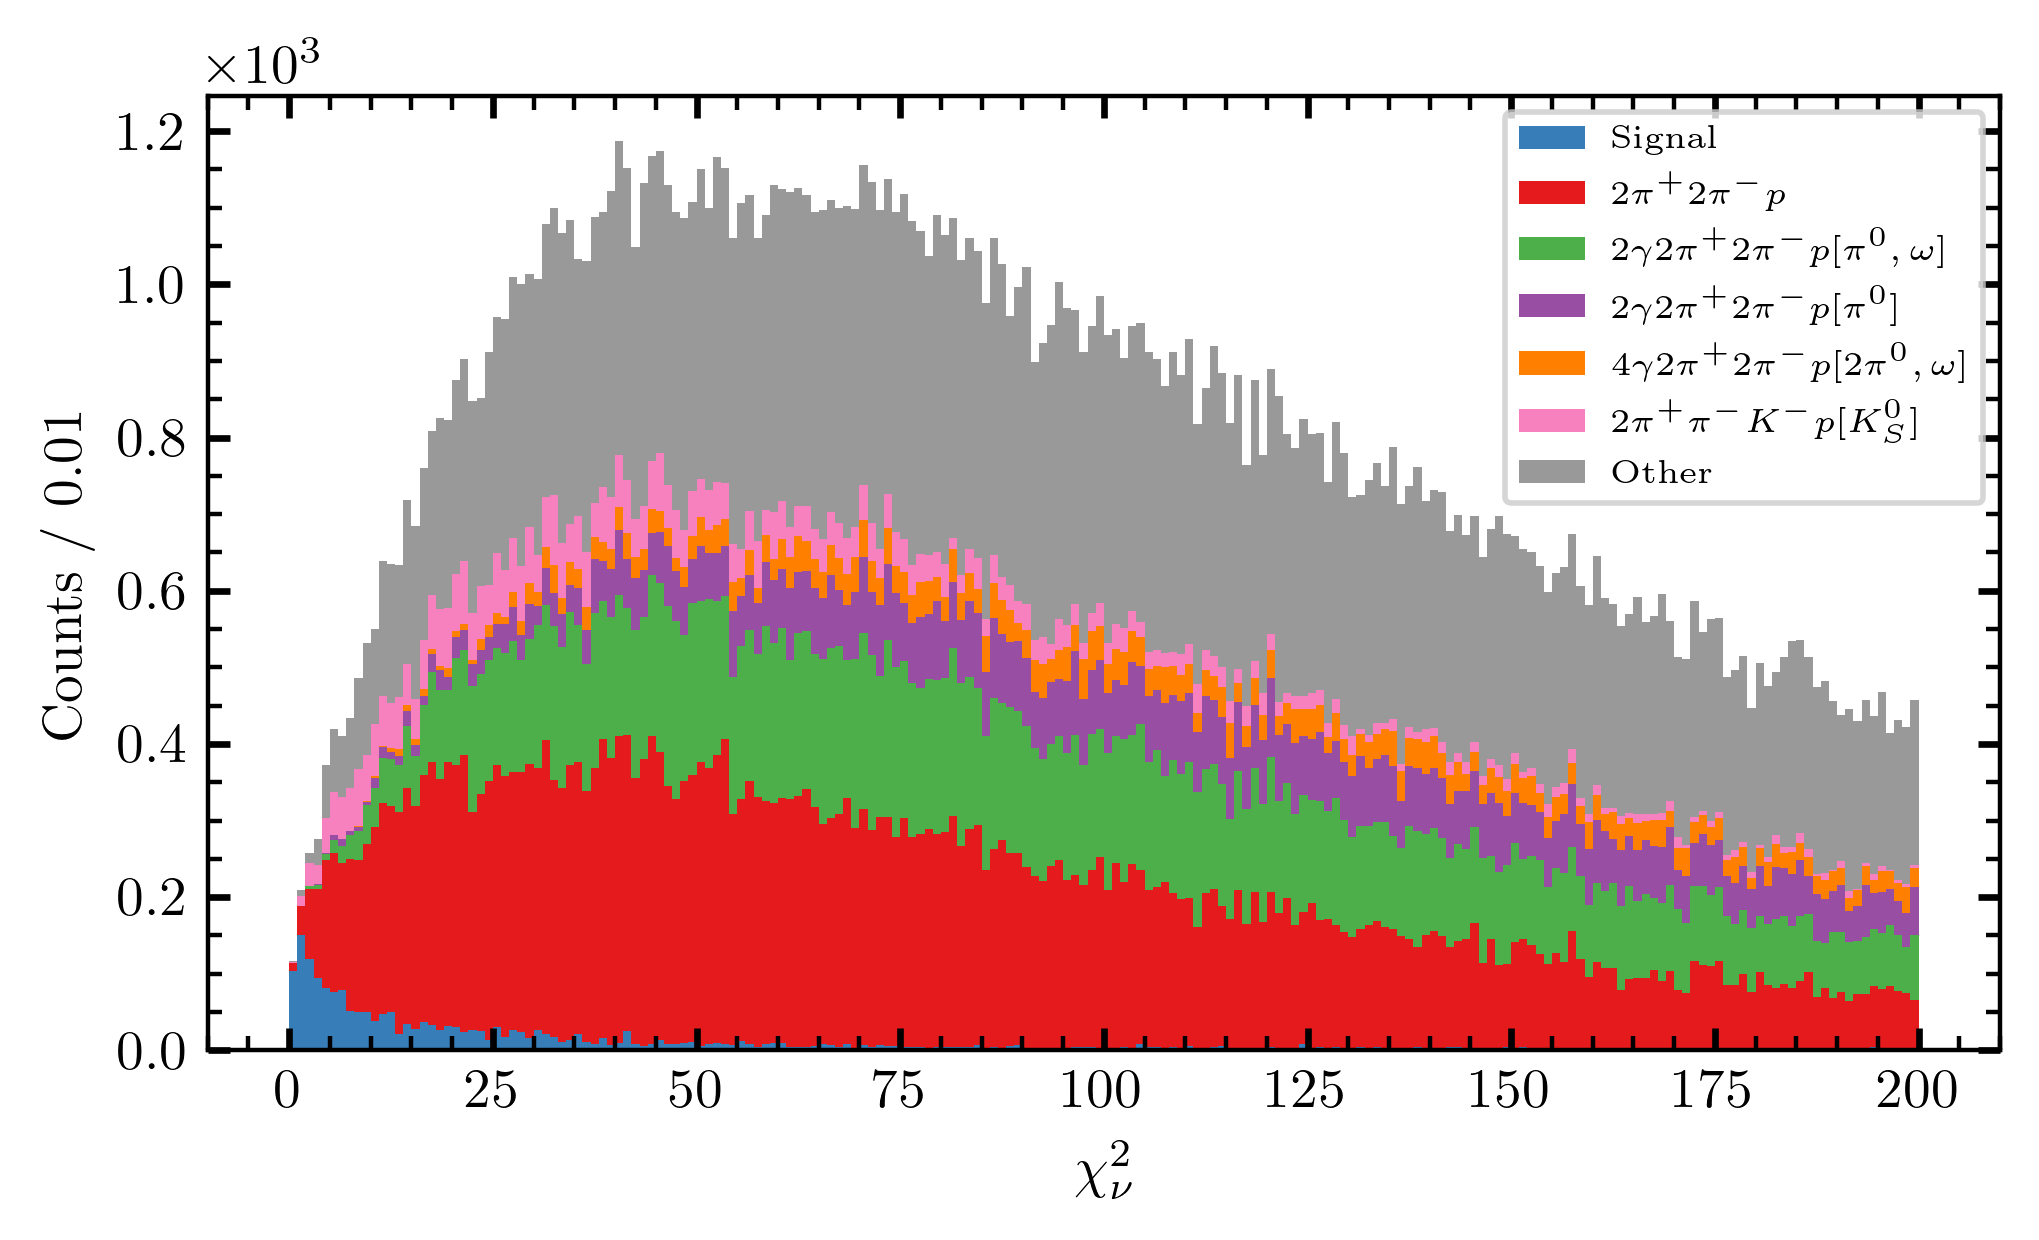
\includegraphics[width=0.8\textwidth]{figures/bggen_chisqdof.png}
  \end{center}
  \caption{The reduced $\chi^2$ statistic of the GlueX kinematic fit for the \texttt{bggen} simulation. The stacked histogram contains the signal channel, $K_S^0K_S^0$ as well as the five most prominent background components.}\label{fig:bggen-chisqdof}
\end{figure}

We will first look at the performance of the GlueX kinematic fit on \texttt{bggen} data in \Cref{fig:bggen-chisqdof}. In this plot, we see the signal, which predictably peaks at $\chi^2_\nu \sim 1$, as well as several background topologies. These topologies are labeled by their final state along with any intermediate decaying resonances in square brackets. The top five potential backgrounds, in order of the size of their contribution after reconstruction, are as follows. First, $2\pi^+2\pi^- p$ shares the final state of the signal channel but does not contain any $K_S^0$ intermediate decays. Second, $2\gamma 2\pi^+ 2\pi^- p [\pi^0, \omega]$ contains an $\omega$ which decays to $\pi^+\pi^-\pi^0$, followed by the $\pi^0$ decaying to $2\gamma$. The addition of extra photons is common in these backgrounds, since missing the photon detections makes the final state identical to the signal. The next two reactions, $2\gamma 2\pi^+ 2\pi^- p [\pi^0]$ and $4\gamma 2\pi^+ 2\pi^- p [2\pi^0, \omega]$ both include an undetected $\pi^0$. Finally, $2\pi^+\pi^- K^- p[K_S^0]$ contains a $K^-$ which is mistakenly identified as a $\pi^-$.

It seems sensible to make a cut on the $\chi^2_\nu$ of the kinematic fit, since the signal is clearly favored at lower values. Below $\chi^2_\nu < 10$, the background topologies are dominated by the $4\pi$ channel which does not contain kaons. As such, this source of background will be our primary focus for removal.
